\begin{figure}
\centering
\begin{tabular}{cc}
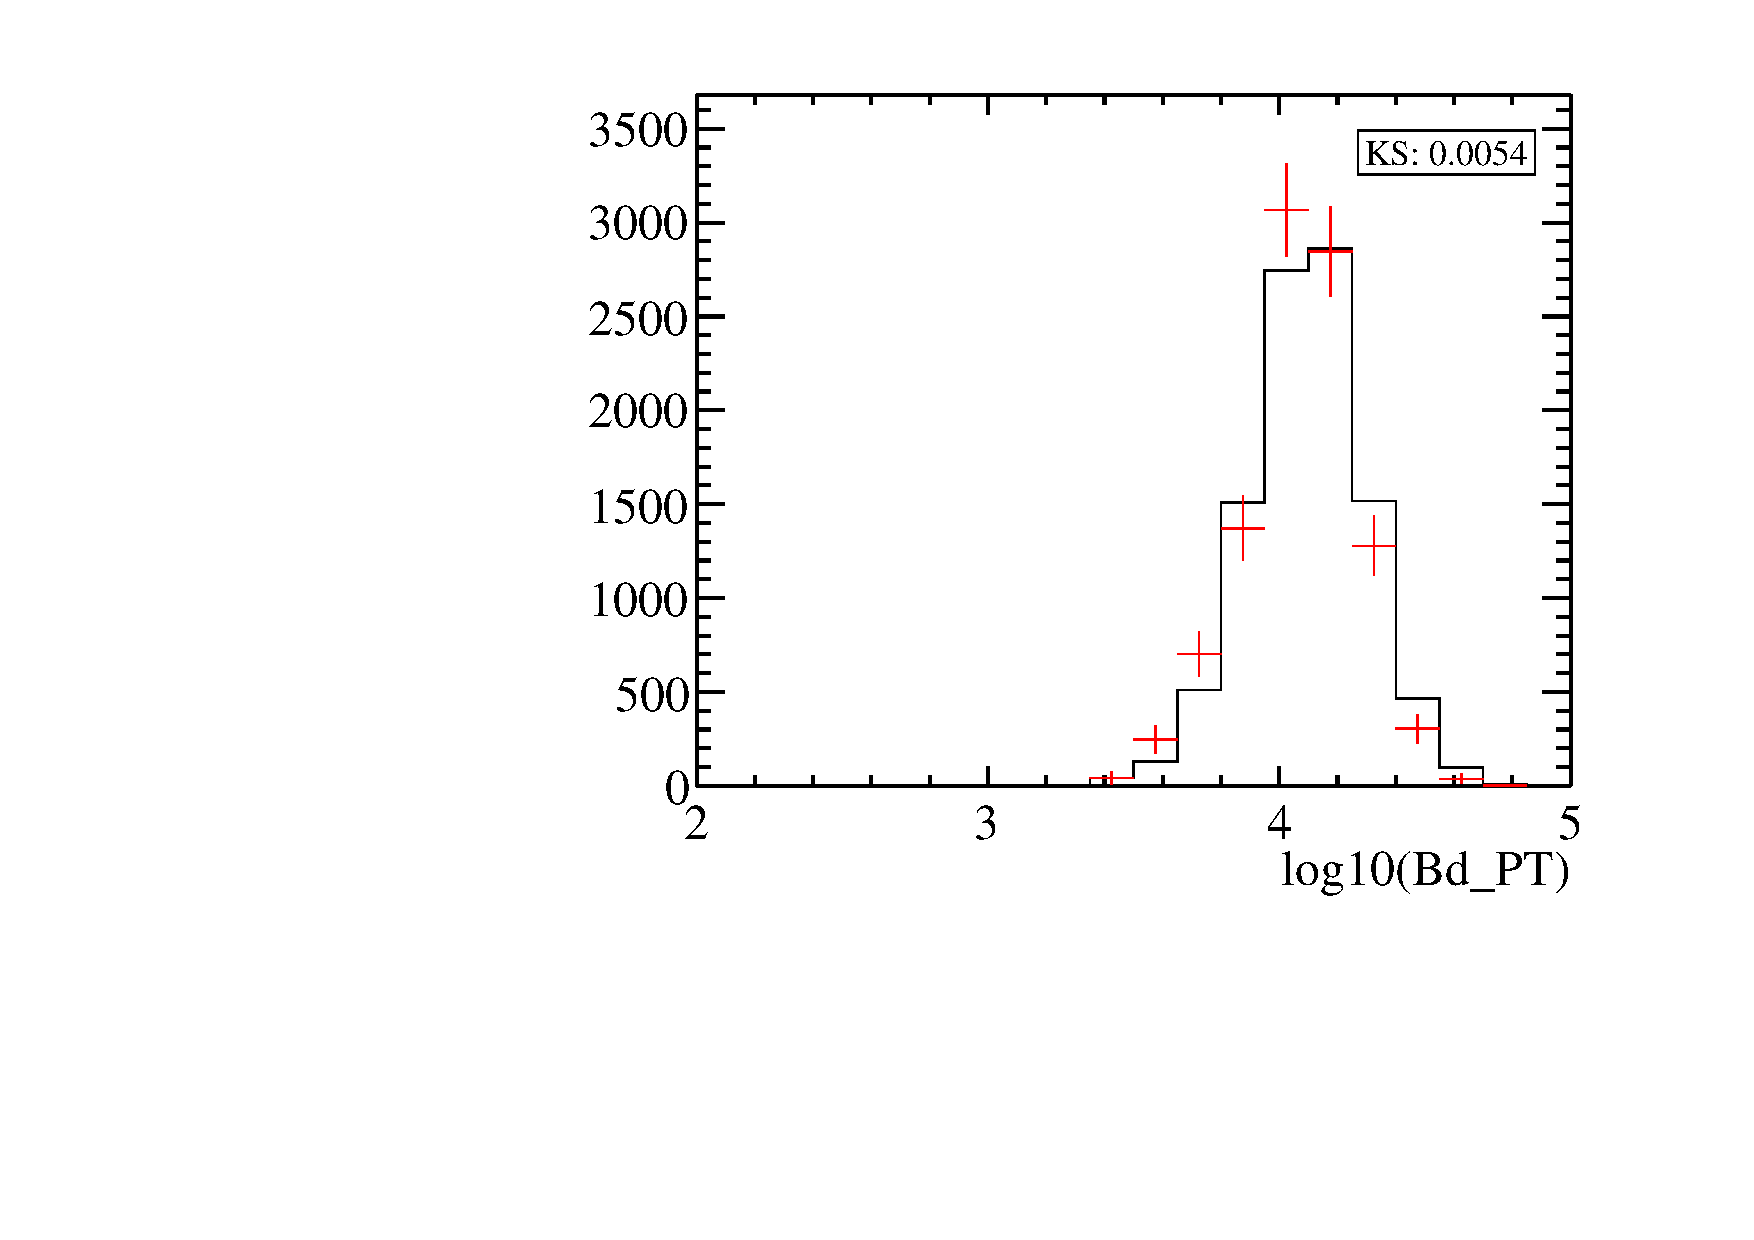
\includegraphics[width=0.3\textwidth]{ANA_resources/Plots/Monte_carlo/data_vs_MC//Kpipipi/log10(Bd_PT)_2016.pdf} & 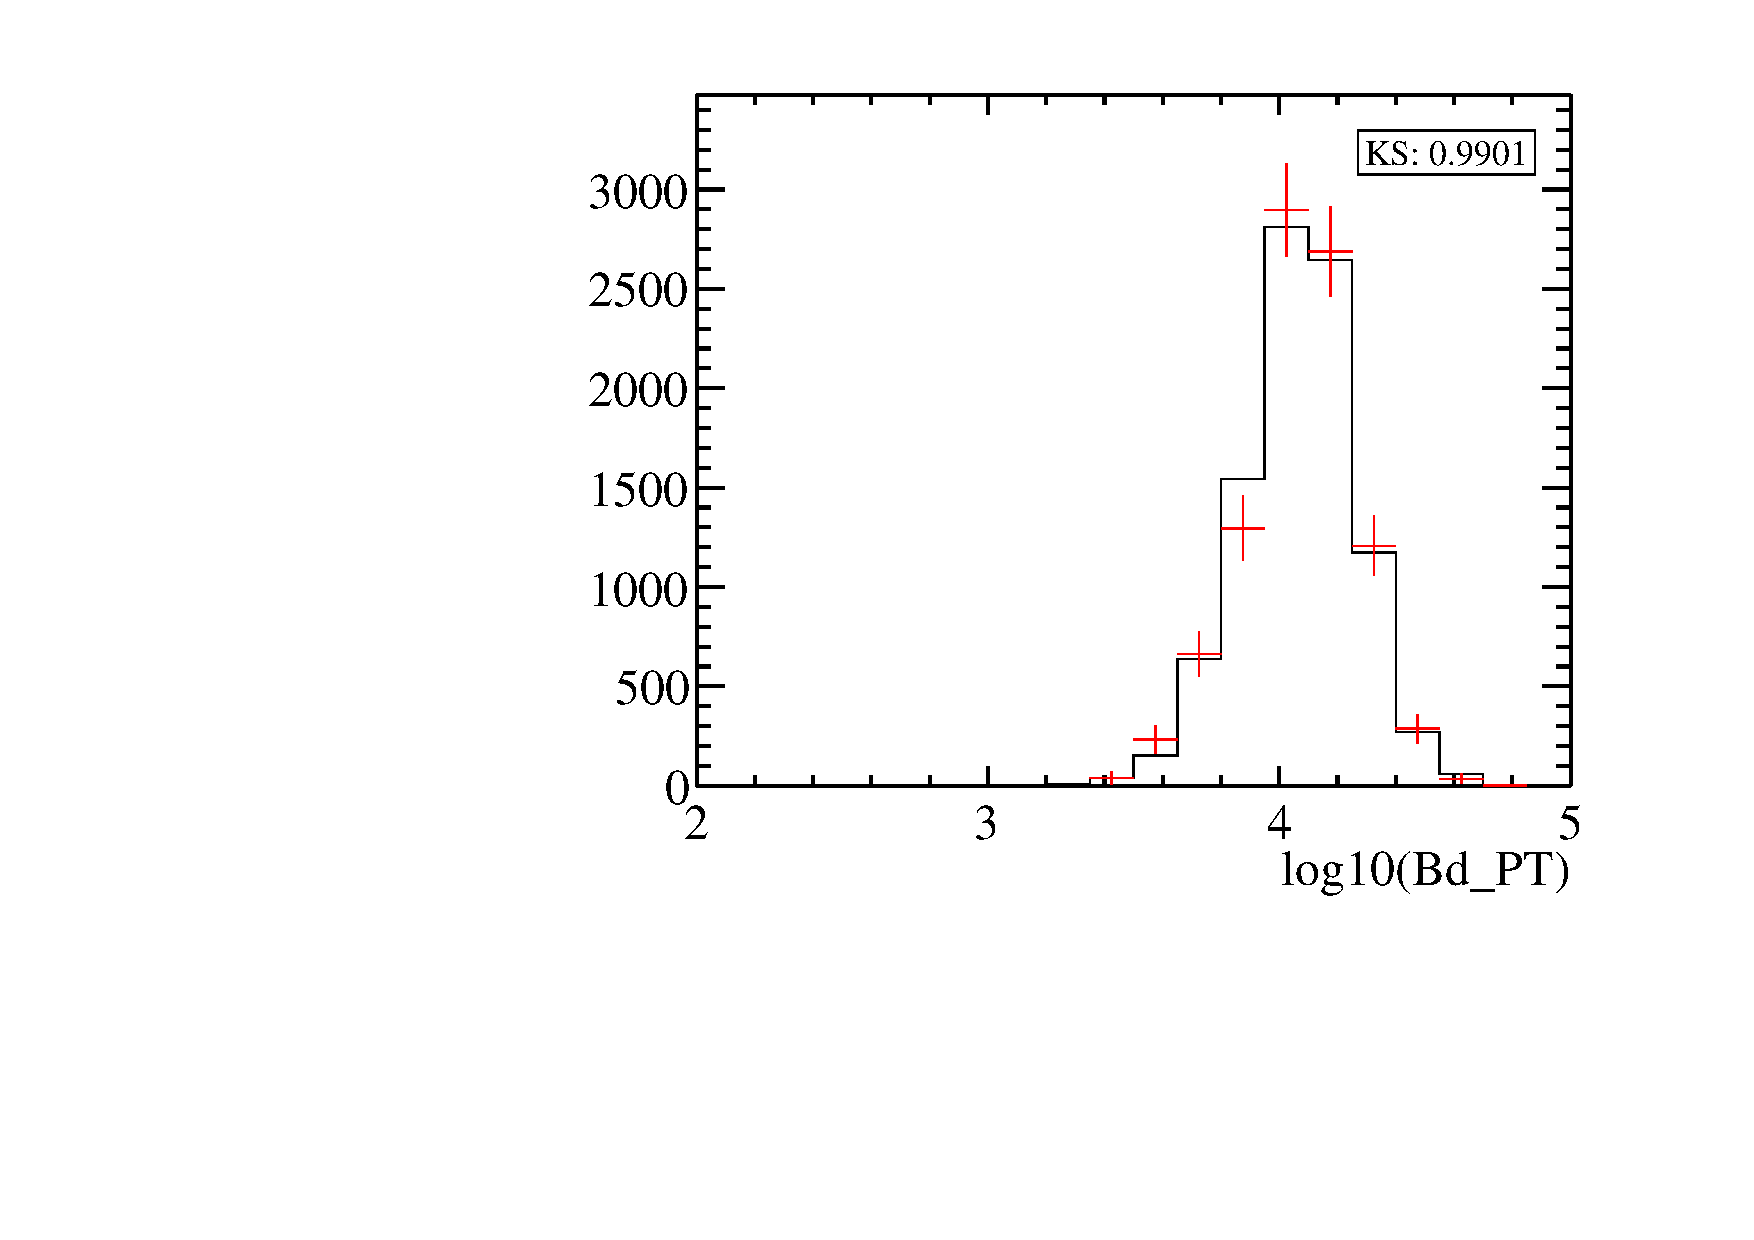
\includegraphics[width=0.3\textwidth]{ANA_resources/Plots/Monte_carlo/data_vs_MC/weight/Kpipipi/log10(Bd_PT)_2016.pdf} \\
\subfloat[][Unweighted MC]{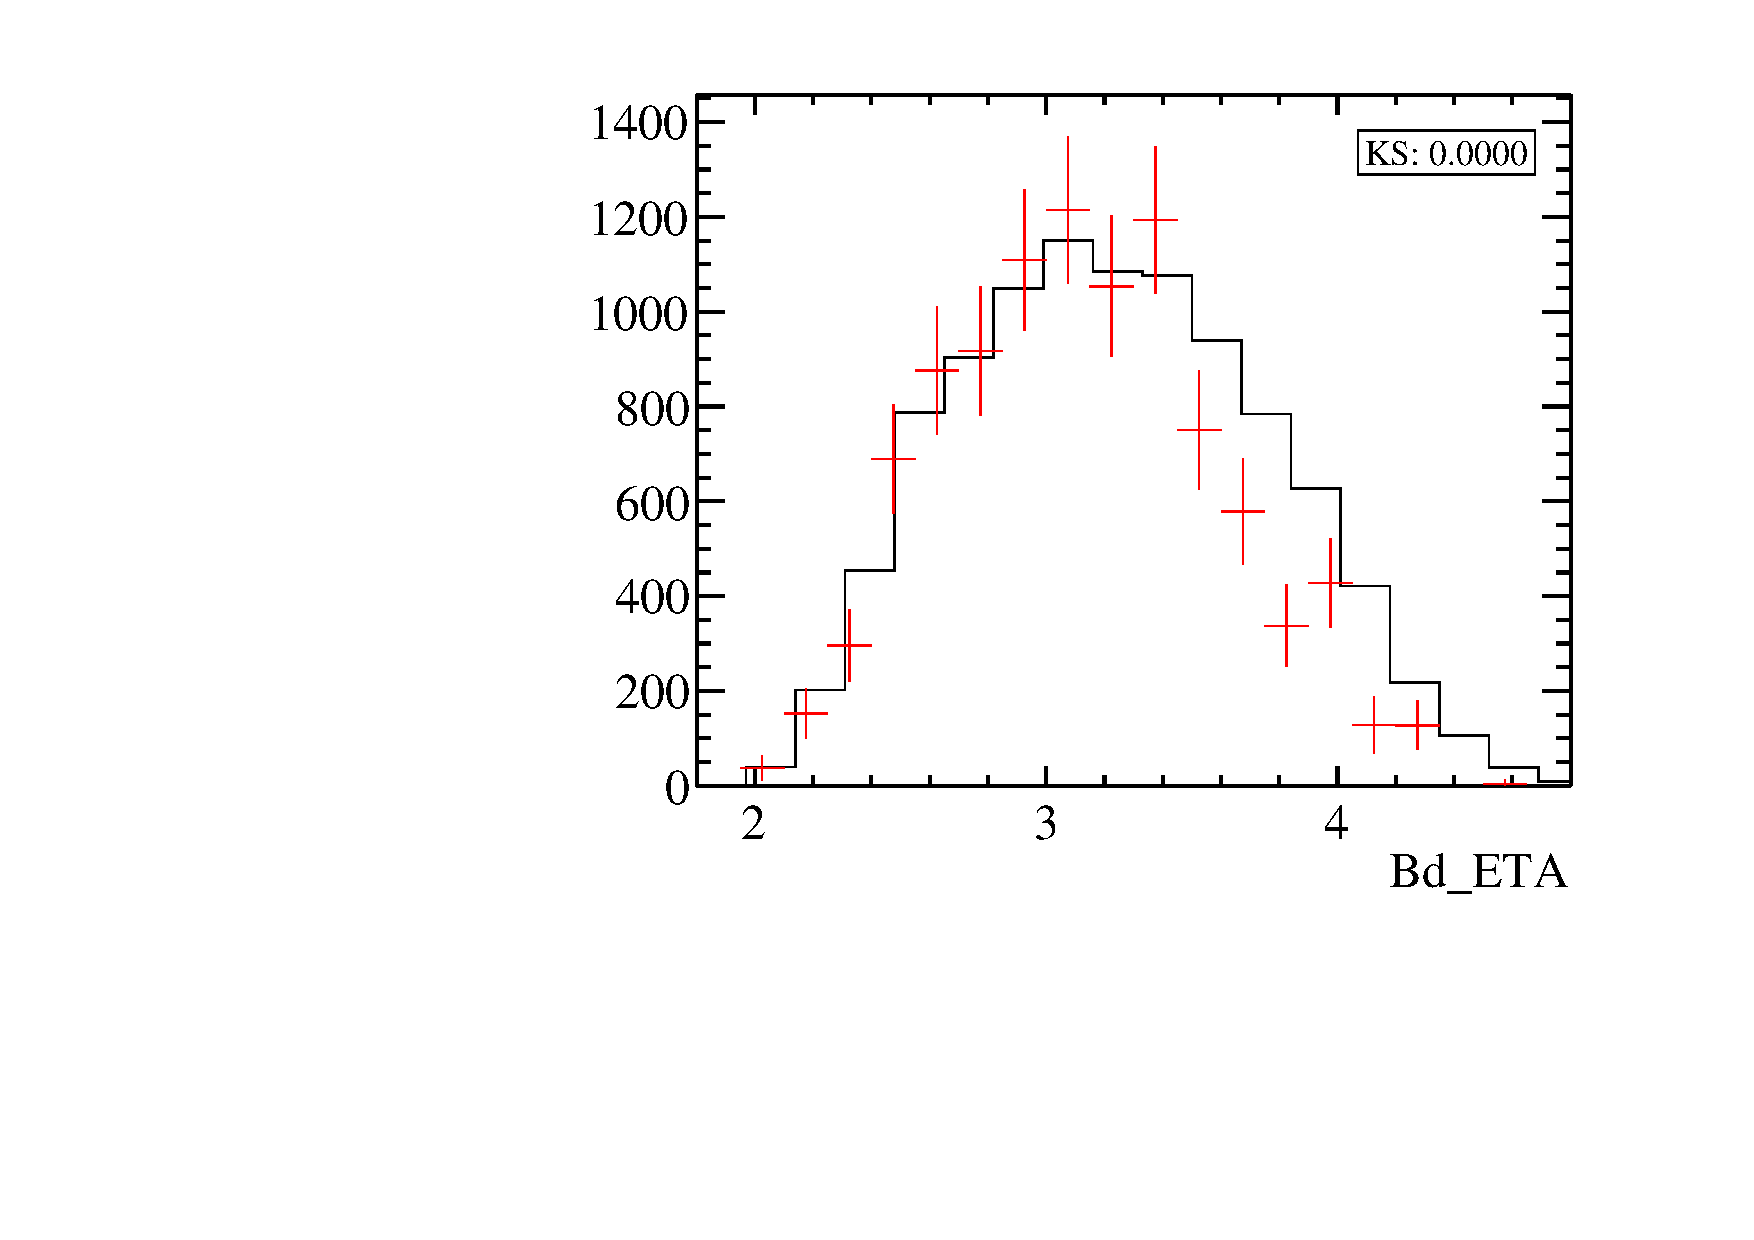
\includegraphics[width=0.3\textwidth]{ANA_resources/Plots/Monte_carlo/data_vs_MC//Kpipipi/Bd_ETA_2016.pdf}} & \subfloat[][Weighted MC]{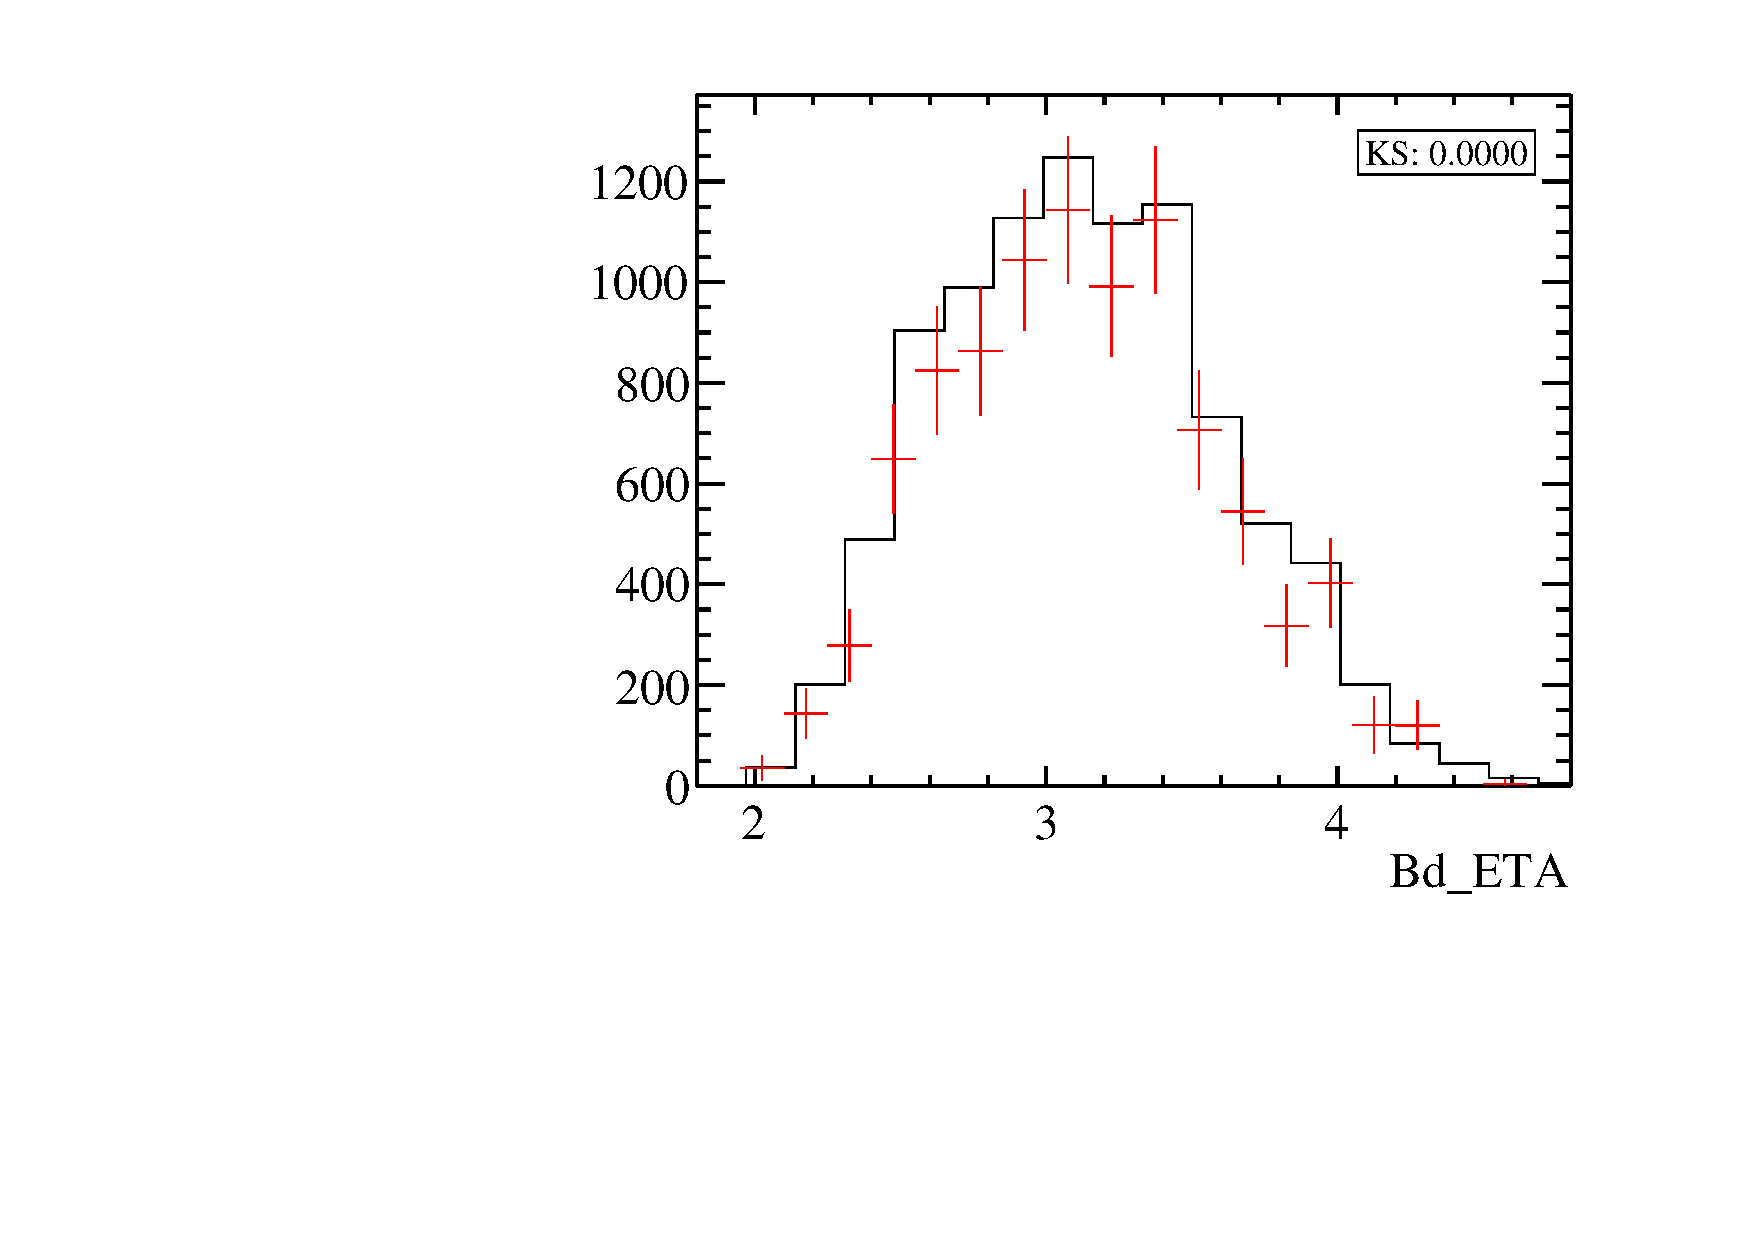
\includegraphics[width=0.3\textwidth]{ANA_resources/Plots/Monte_carlo/data_vs_MC/weight/Kpipipi/Bd_ETA_2016.pdf}} \\
\end{tabular}
\caption{Comparison of sWeighted 2016 data (red points) and Monte Carlo (black histogram) in the $K\pi\pi\pi$ mode for the $B^0$ $p_\mathrm{T}$ (above) and $\eta$ (below), before and after the MC is reweighted to match the data in these two variables.}
\label{fig:reweighting_Kpipipi}
\end{figure}
